% 02/01 changed according to ref No.2
% 02/05 changed from .emf to n.png
% 03/06 English

%%%%%%%%%%%%%%%
%Intruduction%%
%%%%%%%%%%%%%%%
\chapter{Introduction}
\pagenumbering{arabic}

Most of the existing research papers on optimal trading such as Black and Litterman (1991) analyze how informed traders (traders with specific information) construct trading strategies based on their price prediction because the investment performance was considered to be explained mostly by the degree to which the prediction was correct.  However, as the investment business becomes increasingly competitive, it has turned out that the trade execution also significantly affects investment performance.  As a result, many practitioners have started recognizing trade execution as an independent task.  For example, the responsibilities of fund managers and traders are clearly separated in most institutional investors. Principal trades in which security brokers take responsibility of trade execution have become popular for complicated trading needs while execution risk remains investors' responsibility in conventional agency trades.  In contrast, few theoretical research papers can be found about trade execution.  Therefore, this study analyzes the optimal trade execution strategies that minimize trading costs for uninformed traders (traders without specific information) whose trading needs are given exogenously. 

The behavior of uninformed traders depends more on short-term characteristics of price movement than on any long-term forecast.  Therefore, trade execution strategy is largely affected by the market microstructure, the process and outcomes of exchanging assets among financial intermediations and institutions of exchange.  

According to the ``implementation shortfall method" by Perold (1988), the standard framework of market microstructure analysis, trading costs are defined as difference between the market price at the decision-making and evaluating price, which consists of the executed price of filled order and the evaluating price of unfilled order.  Further, trading costs are decomposed into four components, fixed commisions, timing cost, market impact, and opportunity cost as we see in Figure \ref{fg_i0}.  Among them, timing cost is the difference between market price at the decision-making and order placement, market impact is the difference between market price at the order placement and executed price, which is caused by the relationship between trading volume and price change, and opportunity cost is the difference between the executed price and the evaluating price of unfilled order.  Strictly speaking, the nature of timing cost and opportunity cost is the price movement risk and therefore not necessarily a loss.  However, the price movement risk is often recognized as the cost after being multiplied with a conversion factor, where the factor is a risk premium, because most traders are risk averse.  The trade execution strategy can control any market impact and price movement risk.


\begin{figure}[htbp]
\begin{center}
 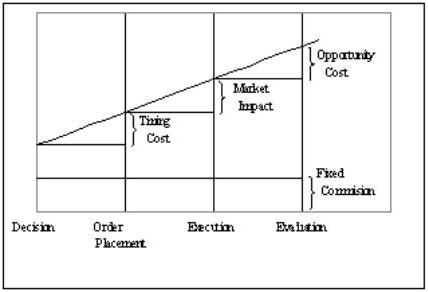
\includegraphics[width=10cm,height=6cm]{fg_i0n.png}
\end{center}
\caption[Decomposition of Implementation Shortfall Method]{{\bf Decomposition of Implementation Shortfall Method.}
\quad Trading costs are decomposed into four components, fixed commisions, timing cost, market impact, and opportunity cost.  ($x$-axis is time and $y$-axis is stock price.)}\label{fg_i0}
\end{figure}

In practice, there are several trading methods in which trading cost occurs in different fashions as shown in Table \ref{table_i1}.  We can also classify these trading methods into fixed-price trades and VWAP trades.  Fixed-price trades are regarded as trades in which execution price is determined explicitly at the trade execution.  Therefore, fixed-price trades include portfolio and block trades, market orders, and limit orders.  Since fixed-price trades tend to suffer larger market impact, execution of large trades should be divided into small orders.  However, fixed-price trades are frequently used by traders who can monitor and respond to the market quickly because traders can optimise fixed-price trades strategy explicitly.

Alternatively, VWAP trades are the second best approach because VWAP trades provide small trading costs and low price movement risks while not necessarily being optimal.  Although VWAP trades cannot be submitted and cancelled quickly because counterparts must agree with the terms and conditions of VWAP before the trades, VWAP trades are convenient methods for certain traders such as foreign investors and individual investors.  Therefore, there are mainly two approaches for saving trading costs: 
\begin{enumerate}
\item To balance the market impact and volatility risk by referring to a fixed price in portfolio or block trades.
\item To mitigate the impact of trades by referring to a volume weighted average price (VWAP henceforth) in VWAP trades.  
\end{enumerate}
These approaches are chosen according to trade size, traders' objectives, circumstances, and so forth.  For example, while Approach 1 has a direct effect on cost reduction, implementation has to be closely monitored during execution.  Therefore, foreign investors rather prefer Approach 2 in order to avoid market impact by completion of large orders under time difference .  Figure \ref{fg_i1} shows a sample flow chart for a choice of trading approaches and methods.

\begin{table}[htbp]
\begin{flushleft}
\begin{tabular}{|l||c|c|c|c|c|l} \hline
 & \multicolumn{4}{c|}{Cost} & & \quad \\ \cline{2-5}
 & Commission & Timing  & Market & Opportunity & Stability / & \quad \\
 & & cost & impact & cost & transparency & \\ \hline
 (Agency trade) & & & & & & \\
 Market order & medium & small & large & small & bad & \\
 Limit order & medium & small & small & large & good & \\
 VWAP trade & medium & medium & small--large & small & good--moderate & \\ \hline
 (Principal trade) & & & & & & \\
 Portfolio trade & large & large & N.A.\ & N.A.\ & moderate & \\
 Block trade & large & small & N.A.\ & N.A.\ & moderate & \\
 VWAP trade & medium & medium & small--large & N.A.\ & good--moderate & \\ \hline
\end{tabular}
\end{flushleft}

\begin{flushright}
\begin{tabular}{l|c|c|c||r|} \hline
 \quad & & & & \\
 & Handling / & Competitiveness & Others & \\
 & optimality & & & \\ \hline
 & & & & (Agency trade) \\
 & bad & bad & & Market order \\
 & good & bad & & Limit order \\
 & good & moderate & measure performance & VWAP order \\ \hline
 & & & & (Principal trade) \\
 & good & good & & Portfolio trade \\
 & good & good & & Block trade \\
 & moderate & good & & VWAP trade \\ \hline
\end{tabular}
\end{flushright}
\caption[Comparison of trading method]{{\bf Comparison of trading method.}
 \quad This table shows the advantages and disadvantages of the trading methods.
 Trading cost is decomposed according to the implementation shortfall method.
 Stability means that it is hard to affect the execution price by instantaneous supply and demand.
 Transparency means that execution price is hard to manipulate.
 Handling means that it is easy to add discretion.
 Optimality means that optimal execution can be expected.
 Competitiveness means that commission is competitive.}
\label{table_i1}
\end{table}

\begin{figure}[htbp]
\def\backsp{\hspace*{-1.5mm}}
\footnotesize{
%\[
\framebox[16.7cm][l]{
${\displaystyle
 \begin{array}{l}
 \quad \\
 \backsp\mbox{Trading Needs}
 \left\{
  \begin{array}{l}
   \backsp\mbox{Time difference}
   \left\{
    \begin{array}{l}
     \backsp\mbox{Large Trade}
     \left\{
      \begin{array}{ll}
       \backsp\mbox{Completion Required} & \rightarrow \mbox{\bf VWAP Trade} \\
       \backsp\mbox{Completion Not Required} & \rightarrow \mbox{\bf Limit Order}
      \end{array}
     \right.
     \\
     \\
     \backsp\mbox{Small Trade}
     \left\{
      \begin{array}{ll}
       \backsp\mbox{Completion Required} & \rightarrow \mbox{{\bf VWAP Trade} or {\bf Market Order}} \\
       \backsp\mbox{Completion Not Required} & \rightarrow \mbox{{\bf Limit Order} or {\bf Market Order}}
      \end{array}
     \right.
    \end{array}
   \right.
   \\
   \\
   \backsp\mbox{No Time difference}
   \left\{
    \begin{array}{l}
     \backsp\mbox{Confident in Execution}
     \left\{
      \begin{array}{ll}
      \multicolumn{2}{l}{
       \backsp\mbox{Large Trade}
       \left\{
        \begin{array}{ll}
         \backsp\mbox{Small Tracking Error} & \rightarrow \mbox{\bf Portfolio Trade} \\
         \backsp\mbox{Large Tracking Error} & \rightarrow \mbox{\bf Block Trade}
        \end{array}
       \right.}
       \\
       \backsp\mbox{Medium Trade} & \rightarrow \mbox{\bf VWAP Trade} \\
       \backsp\mbox{Small Trade} & \rightarrow \mbox{\bf Market Order}
      \end{array}
     \right.
     \\
     \\
     \backsp\mbox{Unconfident in Execution}
     \left\{
      \begin{array}{ll}
       \backsp\mbox{Large Trade} & \rightarrow \mbox{\bf Any Trade} \\
       \backsp\mbox{Small Trade} & \rightarrow \mbox{\bf Any Agency Trade}
      \end{array}
     \right.
    \end{array}
   \right.
  \end{array}
 \right.
 \\
 \quad \\
 \end{array}
}$
}
}
\caption[Flow chart for trading method selection]{{\bf Flow chart for trading method selection.}
 \quad This diagram shows a sample flow chart for a selection of the trading methods, based on comparison of the trading
 methods.}\label{fg_i1}
\end{figure}

This study proposes several optimal trade execution strategies based on the both approaches.  In Approach 1, we analyze a long-term execution scheduling problem and short-term order placement problem since it is difficult to analyze Approach 1 as a whole.  Also, in Approach 2, we analyze both static and dynamic optimization since static optimization works well for numerous small orders while dynamic optimization is more suitable for few large orders.  Therefore, the four cases below are analyzed in the subsequent chapters.

\bigskip

\noindent 1. Fixed-Price Trade
\begin{itemize}
\item Execution Schedule
\item Order Placement
\end{itemize}
\noindent 2. VWAP Trade
\begin{itemize}
\item Static Optimization
\item Dynamic Optimization
\end{itemize}

In practice, all securities trading are carried out through some type of trade execution, regardless of recognition.  At execution, one of the four approaches above is chosen according to the assets' characteristics and traders' objectives and circumstances.  In order to make an appropriate choice, traders have to deeply understand the nature of the alternatives.  

Although a few analyses have been made about the optimal trade execution based on findings of market microstructure, this study derives the optimal execution strategy in both fixed-price trades and VWAP trades, analyzes their characteristics, and provides guidance to the selection of these approaches.  Therefore, an extensive range of applications can be expected for any security trading activity.


\section{Fixed-Price Trade}\label{sec_i1}
\subsection{Execution Schedule}\label{sec_i11}
Konishi and Makimoto (2001) and Chapter \ref{chap_b} of this study, Optimal Slice of a Block Trade, analyze the static optimal execution schedule of fixed-price trades by variational methods.  Traders generally suffer large market impact in immediate execution while they avoid price movement risk.  Therefore, block trades are executed over a considerable duration to balancing market impact and price movement risk.  This study sets objective function as the sum of linear market impact and price movement risk multiplied by a conversion factor.  This value has two economic insights: total cost for traders where the conversion factor is the risk premium, the extent of risk averseness, and value at risk (VaR) for risk managers where the conversion factor is set according to the confidence interval.  This study then, derives analytically the minimal trading cost strategy of liquidation of a portfolio by variational methods.  VaR type risk measurement is widely used because the economic implication is intuitive and because risks of different assets are comparable.  However, since VaR cannot be additive in time, we employ static optimization but not dynamically optimizing.  

The optimal strategies derived by existing studies such as Almgren and Chriss (1999) have the unrealistic property that the time scale of optimal trading is independent of the initial portfolio size although intuition suggests that larger portfolios should trade more slowly and that total execution costs should grow superlinearly with portfolio size.  In contrast, our model has several advantages over existing studies.  First, we succeeded in making optimal execution duration an endogenous increasing function of whole trading size.  Second, the transaction cost of our strategy grows superlinearly with whole trading size, consistent with intuition.  Third, our results are immediately applicable to existing risk management frameworks and provides an explicit solution for minimum liquidity adjusted VaR (L-VaR).  Although this study uses an example of liquidation of a block of common stock, results can also be extended over wider problems on liquidation of any large block of assets.


\subsection{Order Placement}\label{sec_i12}
Chapter \ref{chap_l} of this study, Selection of Market and Limit Order, analyzes the dynamic optimal order placement strategy of fixed-price trades by dynamic programming.  Market and limit orders are frequently submitted and canceled and sometimes switched with each other as market price moves and probability of limit order execution changes.  However, since the execution price and volume of limit orders are non-linear, the economic effect and the optimal order placing strategy is not trivial, and few preceding studies can be found.  Therefore, this study analyses the optimal selection of market and limit orders in a series of single price batch auctions when the expectation of the limit order book is given.  

This study derives the analytical solution of a single limit order model for risk neutral traders by dynamic programming, and then extends the result for risk averse traders.  We find that the limit order size is independent of the whole trade size while the limit order price and the market order size are linear functions and that market orders replace limit orders as time passes.  Further, we calculate the economic value of monitoring the limit order book.


\section{VWAP Trade}\label{sec_i2}
\subsection{Static Optimization}\label{sec_i21}
Konishi (2002) and Chapter \ref{chap_s} of this study, Optimal Slice of a VWAP Trade, analyze the static optimal execution strategy of VWAP trades by an iteration of a single variable optimization.  VWAP trades are overtaking fixed-price trades in numerous trades including foreign investments because of low cost, high transparency, and capability of performance measurement.  Because VWAP trades are labor intensive, automatic execution of a static optimal strategy is often employed for trades with small risk.  

Although a few analyses have been made on the optimal execution of VWAP trades, this study derives analytically the static optimal execution strategy that minimizes the expected squared execution error when market price, price volatility, and market volume is stochastic.  This method is powerful because the optimal execution strategy is determined by an iteration of a single variable optimization, rather than by a multivariable optimization.  Analytical solutions are derived in some cases.  We show that optimal execution times tend to lag behind expected market trading volume distribution since price volatility has a positive correlation with market trading volume.  In a basket trade, execution error can be reduced by spreading out execution times according to the correlation of price movement.  We confirm our theoretical results with actual trading data and simulations.


\subsection{Dynamic Optimization}\label{sec_i22}
Chapter \ref{chap_d} of this study, Dynamic Optimal Slice of a VWAP Trade, further analyzes the dynamic optimal execution strategy of VWAP trades by dynamic programming.  It is feasible to reduce the execution error with a dynamic optimal strategy if a trader picks up a few stocks, monitors VWAP(of the market and the trader), and forecasts the future price movement and trading volume.  This study models the stochastic structure of market volume, and derives an approximation on optimal execution strategy with dynamic programming.  

This analysis confirms execution error reduction by actual trading data.  We find that even if market trading volume surges due to news, or other reasons, the trader should hold his execution rather than follow market execution.  If either buy or sell order is not allowed, execution becomes slower than in the case in which both are allowed.


\bigskip

\section{Closing Remarks}\label{sec_i3}
Although a few analyses have been made about the optimal trade execution based on findings of market microstructure, this study derives the optimal execution strategy in both fixed-price trades and VWAP trades, analyzes their characteristics, and provides guidance to the selection of these approaches.  Therefore, an extensive range of applications can be expected for any security trading activity.

This study is organized as follows.  First, Chapter \ref{chap_r} surveys relevant existing studies.  Chapter \ref{chap_b} to Chapter \ref{chap_d} analyze the optimal execution strategies of the four cases described above.  Finally, Chapter \ref{chap_c} concludes this study.
